\documentclass{article}

\usepackage{graphicx}
\usepackage[a4paper, total={6.5in, 10in}, margin=1.8cm]{geometry}
\usepackage[T1]{fontenc}
\usepackage[french]{babel}
\usepackage{hyphenat}
\usepackage{fancybox}
\usepackage{fancyhdr}
\hyphenation{mate-mática recu-perar}
\usepackage{pifont}
\usepackage{tikz,tikz-3dplot}
\usepackage{siunitx}
\usepackage{etoolbox}
\usepackage{lmodern}
\usepackage{booktabs}
\usepackage{listings}
\usepackage{matlab-prettifier}
% \usepackage[dvipsnames]{xcolor}
\usetikzlibrary{shapes.geometric}
\usetikzlibrary{shapes.symbols}
\usepackage{caption}
\usepackage{subcaption}
\usepackage{cprotect}
\usepackage{tabularx, tabularray}
\usepackage{multirow}
\usepackage{pdfpages}
\usepackage{lastpage}
\usepackage[colorlinks=true, linkcolor=black]{hyperref}
\usepackage{amsmath, amsfonts, amssymb, empheq}
\usepackage{mathtools}
\usepackage{xfrac}


% \renewcommand*{\lstlistlistingname}{Liste des codes sources}
% \renewcommand*{\lstlistingname}{Code source}

\definecolor{font}{RGB}{28, 28, 28}
\definecolor{codegray}{rgb}{0.5,0.5,0.5}
\definecolor{A}{RGB}{245, 87, 146}
\definecolor{B}{RGB}{242, 142, 93}
\definecolor{C}{RGB}{245, 206, 92}
\definecolor{D}{RGB}{159, 210, 108}
\definecolor{E}{RGB}{110, 210, 222}
\definecolor{F}{RGB}{161, 147, 232}
\definecolor{G}{RGB}{85, 83, 88}

\definecolor{Gr}{RGB}{0, 220, 0}
\definecolor{Ye}{RGB}{252, 186, 3}

\lstdefinestyle{prog}{
    style=Matlab-editor,
    basicstyle=\ttfamily\footnotesize\color{font},
    breaklines=true,
    frame=tb,
    numbers=left,
    showlines=true,
    inputencoding=utf8,  % Input encoding
    extendedchars=true,  % Extended ASCII
    literate={
        {á}{{\'a}}1  {é}{{\'e}}1  {í}{{\'i}}1 {ó}{{\'o}}1  {ú}{{\'u}}1
        {Á}{{\'A}}1  {É}{{\'E}}1  {Í}{{\'I}}1 {Ó}{{\'O}}1  {Ú}{{\'U}}1
        {à}{{\`a}}1  {è}{{\`e}}1  {ì}{{\`i}}1 {ò}{{\`o}}1  {ù}{{\`u}}1
        {À}{{\`A}}1  {È}{{\'E}}1  {Ì}{{\`I}}1 {Ò}{{\`O}}1  {Ù}{{\`U}}1
        {ä}{{\"a}}1  {ë}{{\"e}}1  {ï}{{\"i}}1 {ö}{{\"o}}1  {ü}{{\"u}}1
        {Ä}{{\"A}}1  {Ë}{{\"E}}1  {Ï}{{\"I}}1 {Ö}{{\"O}}1  {Ü}{{\"U}}1
        {â}{{\^a}}1  {ê}{{\^e}}1  {î}{{\^i}}1 {ô}{{\^o}}1  {û}{{\^u}}1
        {Â}{{\^A}}1  {Ê}{{\^E}}1  {Î}{{\^I}}1 {Ô}{{\^O}}1  {Û}{{\^U}}1
        {œ}{{\oe}}1  {Œ}{{\OE}}1  {æ}{{\ae}}1 {Æ}{{\AE}}1  {ß}{{\ss}}1
        {ç}{{\c c}}1 {Ç}{{\c C}}1 {ø}{{\o}}1  {Ø}{{\O}}1   {å}{{\r a}}1
        {Å}{{\r A}}1 {ã}{{\~a}}1  {õ}{{\~o}}1 {Ã}{{\~A}}1  {Õ}{{\~O}}1
        {ñ}{{\~n}}1  {Ñ}{{\~N}}1  {¿}{{?`}}1  {¡}{{!`}}1
        {°}{{\textdegree}}1 {º}{{\textordmasculine}}1 {ª}{{\textordfeminine}}1
    }
}
\lstset{style=prog}

\newlength{\larg}
\setlength{\larg}{15.5cm}

\title{
    \Huge {\bf APEX} \\
    \huge Rapport de projet\\
}
\author{Alexis Paillard, Malo Amaranti}  

\makeatletter
\def\@maketitle{
    \begin{center}
    \begin{tabular}{>{\raggedright\arraybackslash}m{0.5\textwidth}
        >{\raggedleft\arraybackslash}m{0.5\textwidth}}
        & \vspace{-1cm}
\includegraphics[width=0.25\textwidth]{image/Logo_Alpha2.png}
    \end{tabular}
    \vspace{1cm}
    % \begin{tabular}{m{0.6\textwidth}m{0.4\textwidth}}
    %     IPSA (Institut Polytechnique des & \\
    %     Sciences Avancées) & \\
    %     63 bvd de Brandbourg & \\
    %     94200 Ivry-sur-Seine &
    % \end{tabular}
    \end{center}
    % \begin{flushright}
    \begin{center}
        {\rule{\larg}{1mm}}\\
        \vspace{3mm}
        \@title
        \vspace{2mm}
        {\rule{\larg}{1mm}}\\
    \end{center}
    % \end{flushright}
    \vspace{1cm}
    \begin{figure}[h]
        \centering
        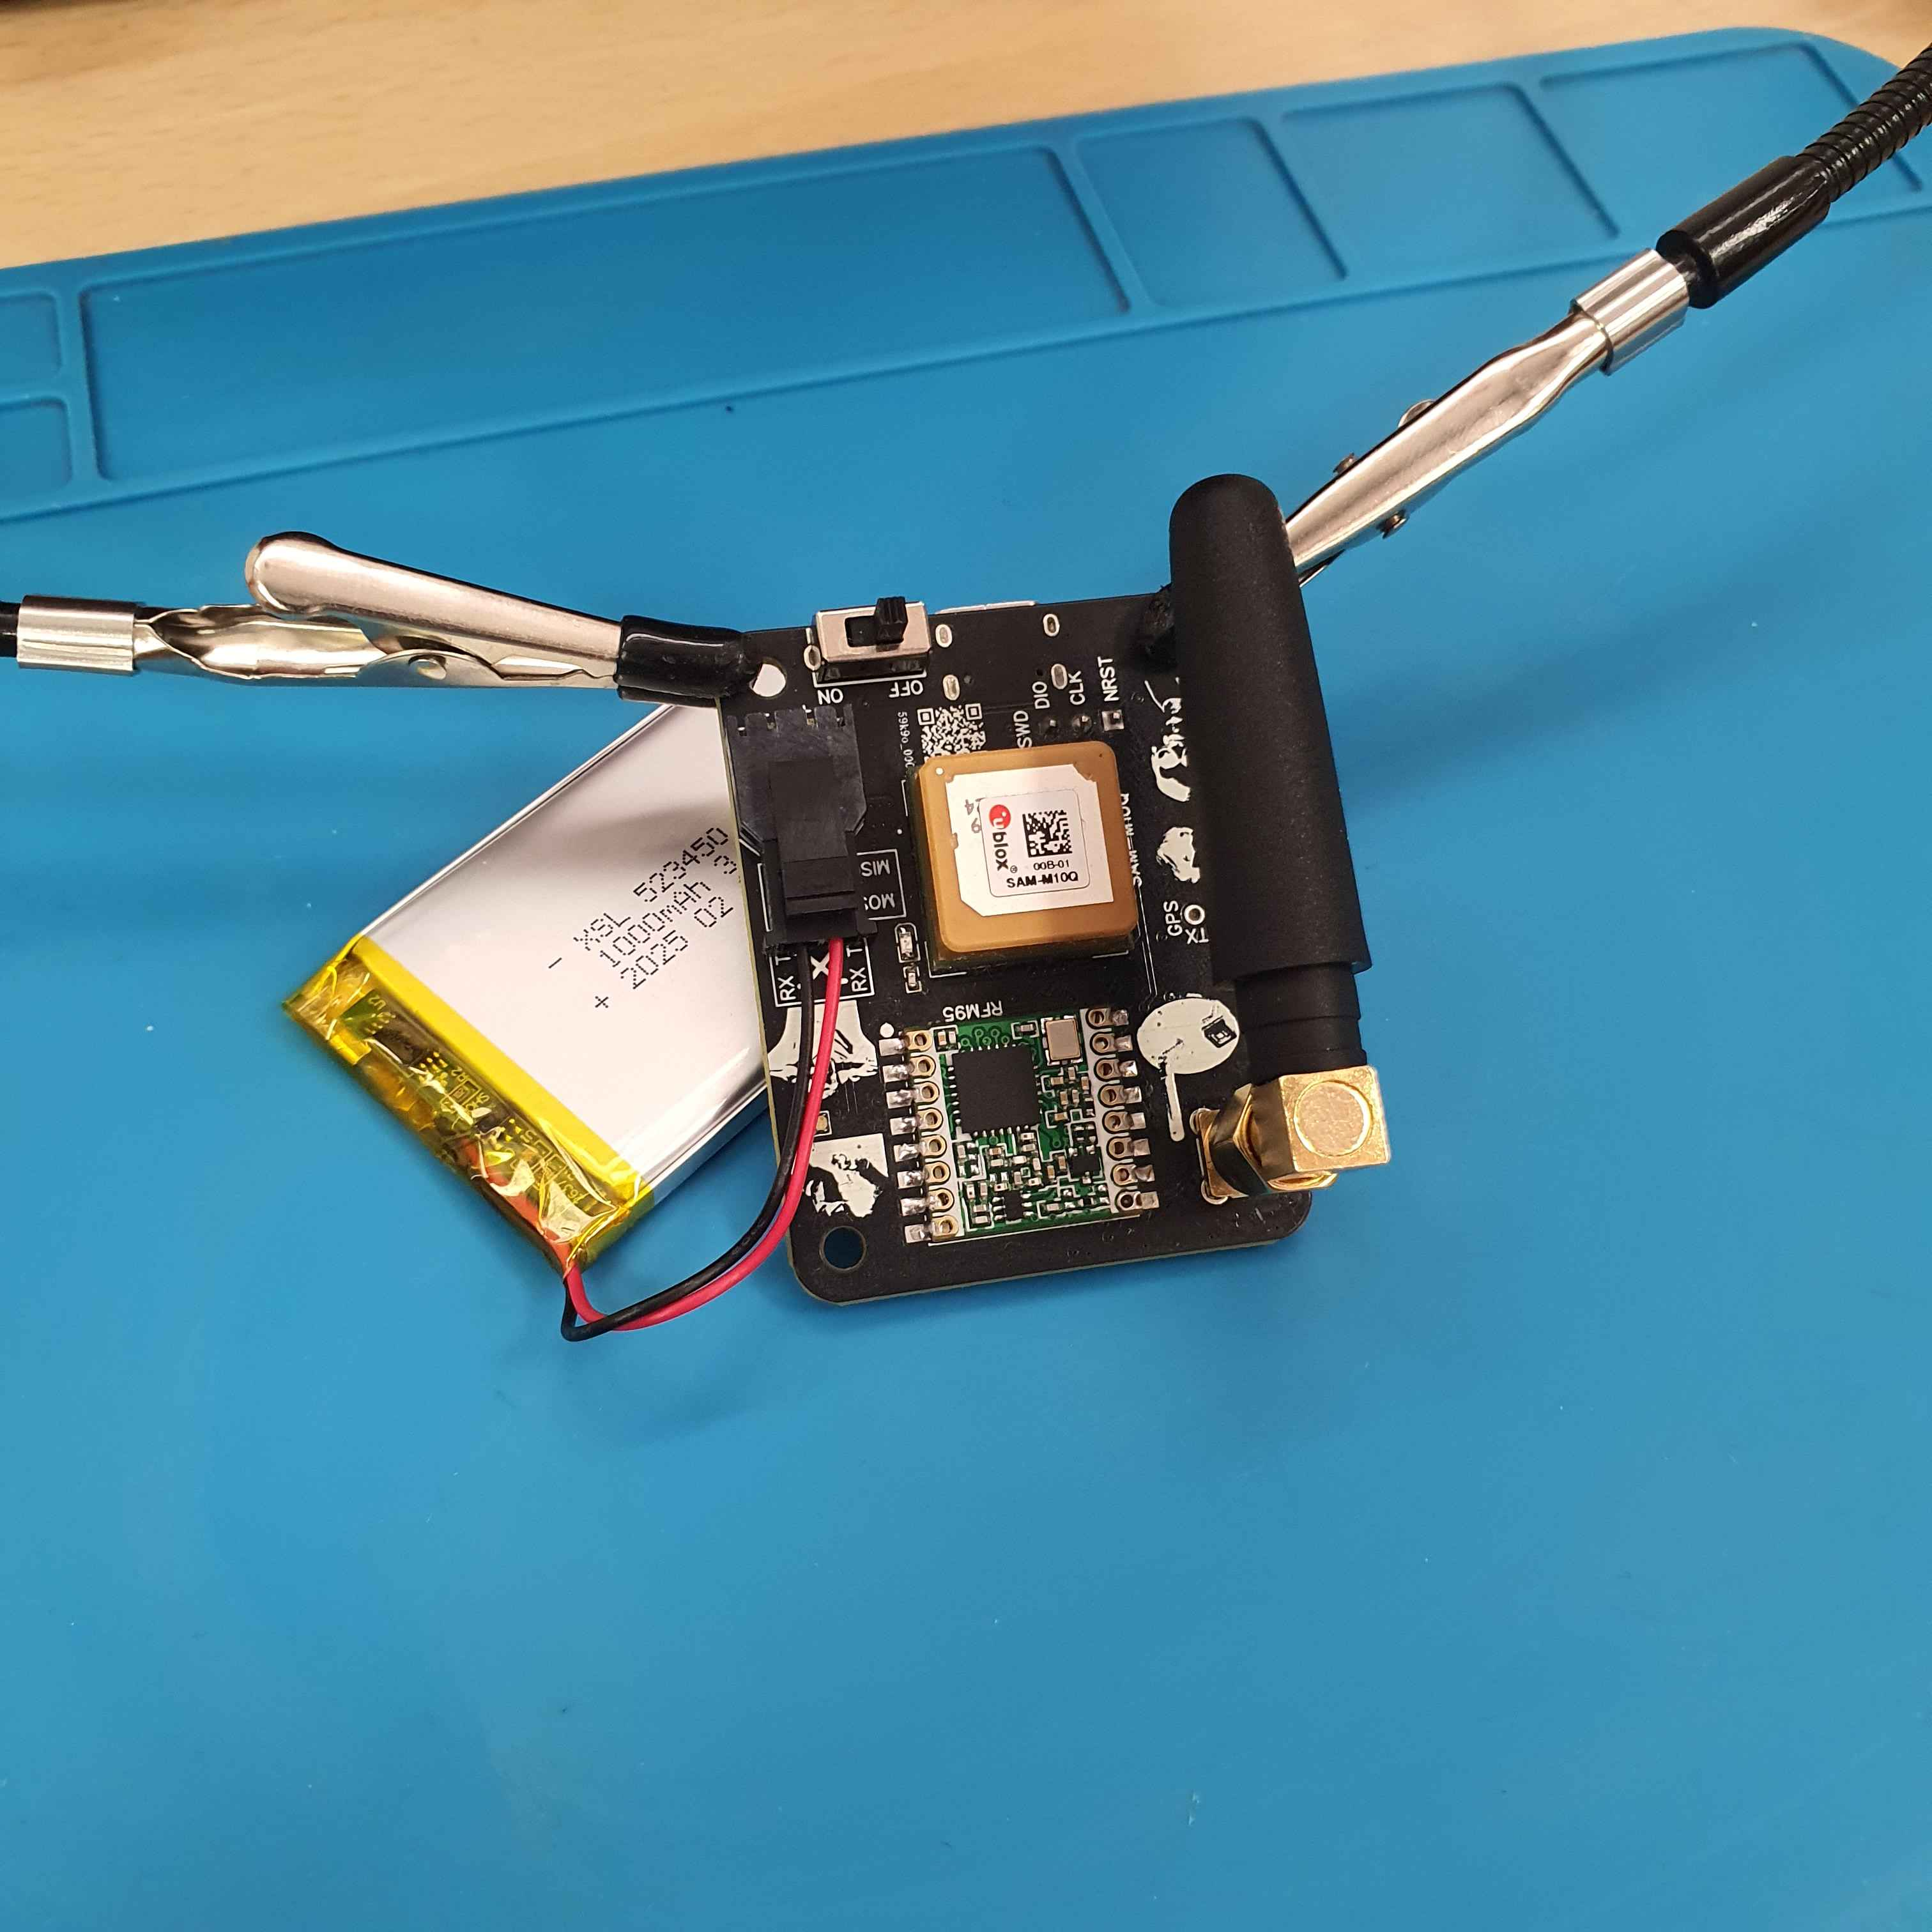
\includegraphics[width=0.60\textwidth]{image/apex_pres.jpg}
        \caption{Module APEX}
    \end{figure}

    \vspace{1cm}

    Membres du projet :\\
    \begin{itemize}
        \item Alexis Paillard
        \item Malo Amaranti
        \item Lucas Pichon
        \item Elouan Fraudet
    \end{itemize}

    \vfill
    \begin{tabular}{>{\raggedright\arraybackslash}m{0.5\textwidth}
        >{\raggedleft\arraybackslash}m{0.5\textwidth}}
         & \@date\\
        \hline
    \end{tabular}
}
\makeatother



\begin{document}

\pagestyle{fancy}
\pagenumbering{arabic}
\fancyhf{} % sets both header and footer to nothing
\renewcommand{\headrulewidth}{0pt} % removes horizontal line
% \fancyhead[R]{\vspace{2cm}\rightmark}
\fancyhead[R]{\rightmark}

%Header and footer images
\AddToShipoutPictureBG{%
  \AtPageUpperLeft{%
    \makebox(\paperwidth,0)[lt]{
\includegraphics[height=1.25cm]{image/AEROIPSA_HEADER.png}}%
  }
  \AtPageLowerLeft{%
    \makebox(\paperwidth,0)[rb]{
\includegraphics[height=1.25cm]{image/AEROIPSA_FOOTER.png}}%
  }%
}


\pagenumbering{gobble}
\maketitle


\newpage


\tableofcontents
\listoffigures

\pagestyle{fancy}
\pagenumbering{arabic}
\fancyhf{} % sets both header and footer to nothing
\renewcommand{\headrulewidth}{0pt} % removes horizontal line
% \fancyhead[R]{\vspace{2cm}\rightmark}
\fancyhead[R]{\rightmark}
\fancyfoot[L]{\thepage/\pageref{LastPage}} 

\newpage

\section{Mise en contexte}
Ce rapport fait l'objet du retour d'expérience sur le projet APEX.\\

Le projet APEX a été réalisé dans le cadre d'un travail réalisé au cours de l'année
scolaire 2024-2025 au sein de l'association de l'AéroIPSA.\\

\subsection*{- L'AeroIPSA}
L'AéroIPSA est une association étudiante de l'école d'ingénieurs IPSA qui conçoit et
réalise entièrement des projets fonctionnels en rapport avec le secteur
aérospatial. Elle rassemble des étudiants autour de projets d'astromodélisme,
principalement de lanceurs, mais aussi de Cansats (micro-satellites atmosphérique).
Cela permet aux différents membres de l'association d'appliquer les notions
apprises durant leur cursus au profit d'un projet d'envergure et d'acquérir les
compétences nécessaires dans leur futur métier d'ingénieur.

\subsection*{- APEX}
APEX est un projet d'électronique se découpant en deux parties : la partie
électronique embarquée et la partie sol. La partie embarquée est un module
électronique de fusée, baptisé "APEX" et servant à collecter des données durant le
vol de la fusée et à les transmettre au sol. La partie sol est une mallette
contenant un ordinateur, une batterie et un récepteur de télémesure appelé
"Station sol". Le projet se base en grande partie sur un projet précédent
baptisé "Unknown".

\subsection*{- Unknown}
Unknown est un projet de module électronique de fusée expérimentale réalisé par
Vincent Fauquembergue et Alexis Paillard et ayant volé sur le projet SP-01 lors de la
campagne de lancmenet du C'space 2024. Les expériences du projet Unknown ont été
les suivantes :
\begin{itemize}
    \item \textbf{Expérience principale} : Relocaliser une fusée après son lancement
    grâce à un module de télémesure LoRa renvoyant les données GNSS tout au long du
    vol.
    \item \textbf{Expérience secondaire} : Réalisation d'une collecte de données
    provenant de nombreux capteurs, barométrique et centrale inertielle, afin de
    reconstituer le vol après récupération des données stockées sur une mémoire
    flash.
\end{itemize}
L'un des objectifs du projet Unknown était de réaliser un module électronique se
voyant plus facilement intégrable dans une fusée amateur. Cela s'est traduit par
l'utilisation d'une seule carte électronique ayant tous ses composants directement
soudés dessus ainsi que l'utilisation d'un microcontrôleur autre que l'Arduino ou
que la Teensy. Le choix fait s'est porté sur un STM32F4 de STMicroelectronics. La
programmation de ce microcontrôleur a été réalisée en C et un bon nombre des
drivers nécessaires ont dû être réadapté par les membres du projet ce qui a permis
d'acquérir de nouvelles compétences en programmation bas niveau.

\subsection*{- Objectifs et enjeux du projet APEX}
Le projet APEX s'inscrit dans la continuité du projet Unknown avec pour objectifs
principaux :
\begin{itemize}
    \item \textbf{Faciliter l'intégration} : Développer un module plus compact et
    modulaire
    \item \textbf{Enrichir les données} : Étendre les capacités de collecte de données
    en ajoutant de nouveaux capteurs et en améliorant la précision des données
    \item \textbf{Augmenter la connectivité} : Ajouter de nouveaux moyens de connexion
    entre le module et d'autres organes de la fusée
    \item \textbf{Maximiser la rapidité d'execution} : Optimiser le code et intégrer des
    techniques de programmation avancées pour garentir une fréquence d'échantillonnage
    élevée tout en gardant une modularité du code
    \item \textbf{Avoir une station sol plus performante} : Développer une station sol
    capable de recevoir les données en temps réel et de les afficher de manière
    compréhensible, intuitive et modulaire afin qu'elle puisse être utilisée
    facilement par les membres de l'association pour d'autres projets
\end{itemize}

\newpage
\section{Module électronique APEX}

\subsection{Présentation du module}

Le module APEX est composé d'une seule carte électronique de forme rectangulaire sur
laquelle sont soudés tous les composants nécessaires à son fonctionnement. Il est conçu
pour être compact permettant une intégration facile dans une fusée ou cansat et est
alimenté par une batterie LiPo 3.7V. Il est équipé de plusieurs capteurs dont un gps,
d'une interfaces de communication physique, d'une mémoire flash pour le stockage des
données, d'un module de télémesure LoRa\texttrademark et d'un microcontrôleur
STM32F411RETx de STMicroelectronics. Le module est programmé en C.

Le coût total d'une carte avec sa batterie, son antenne et tous ces composants s'élève à
110 €. 4 modules ont été commandé ce qui fait que cette partie du projet avait un budget
aloué d'au moins 440 €.\\

La figure \ref{fig:apex} présente le module APEX avec ses composants principaux labelisés.

\begin{figure}[h]
    \centering
    \begin{subfigure}{0.48\textwidth}
        \centering
\begin{tikzpicture}
    \node at (0, 0) {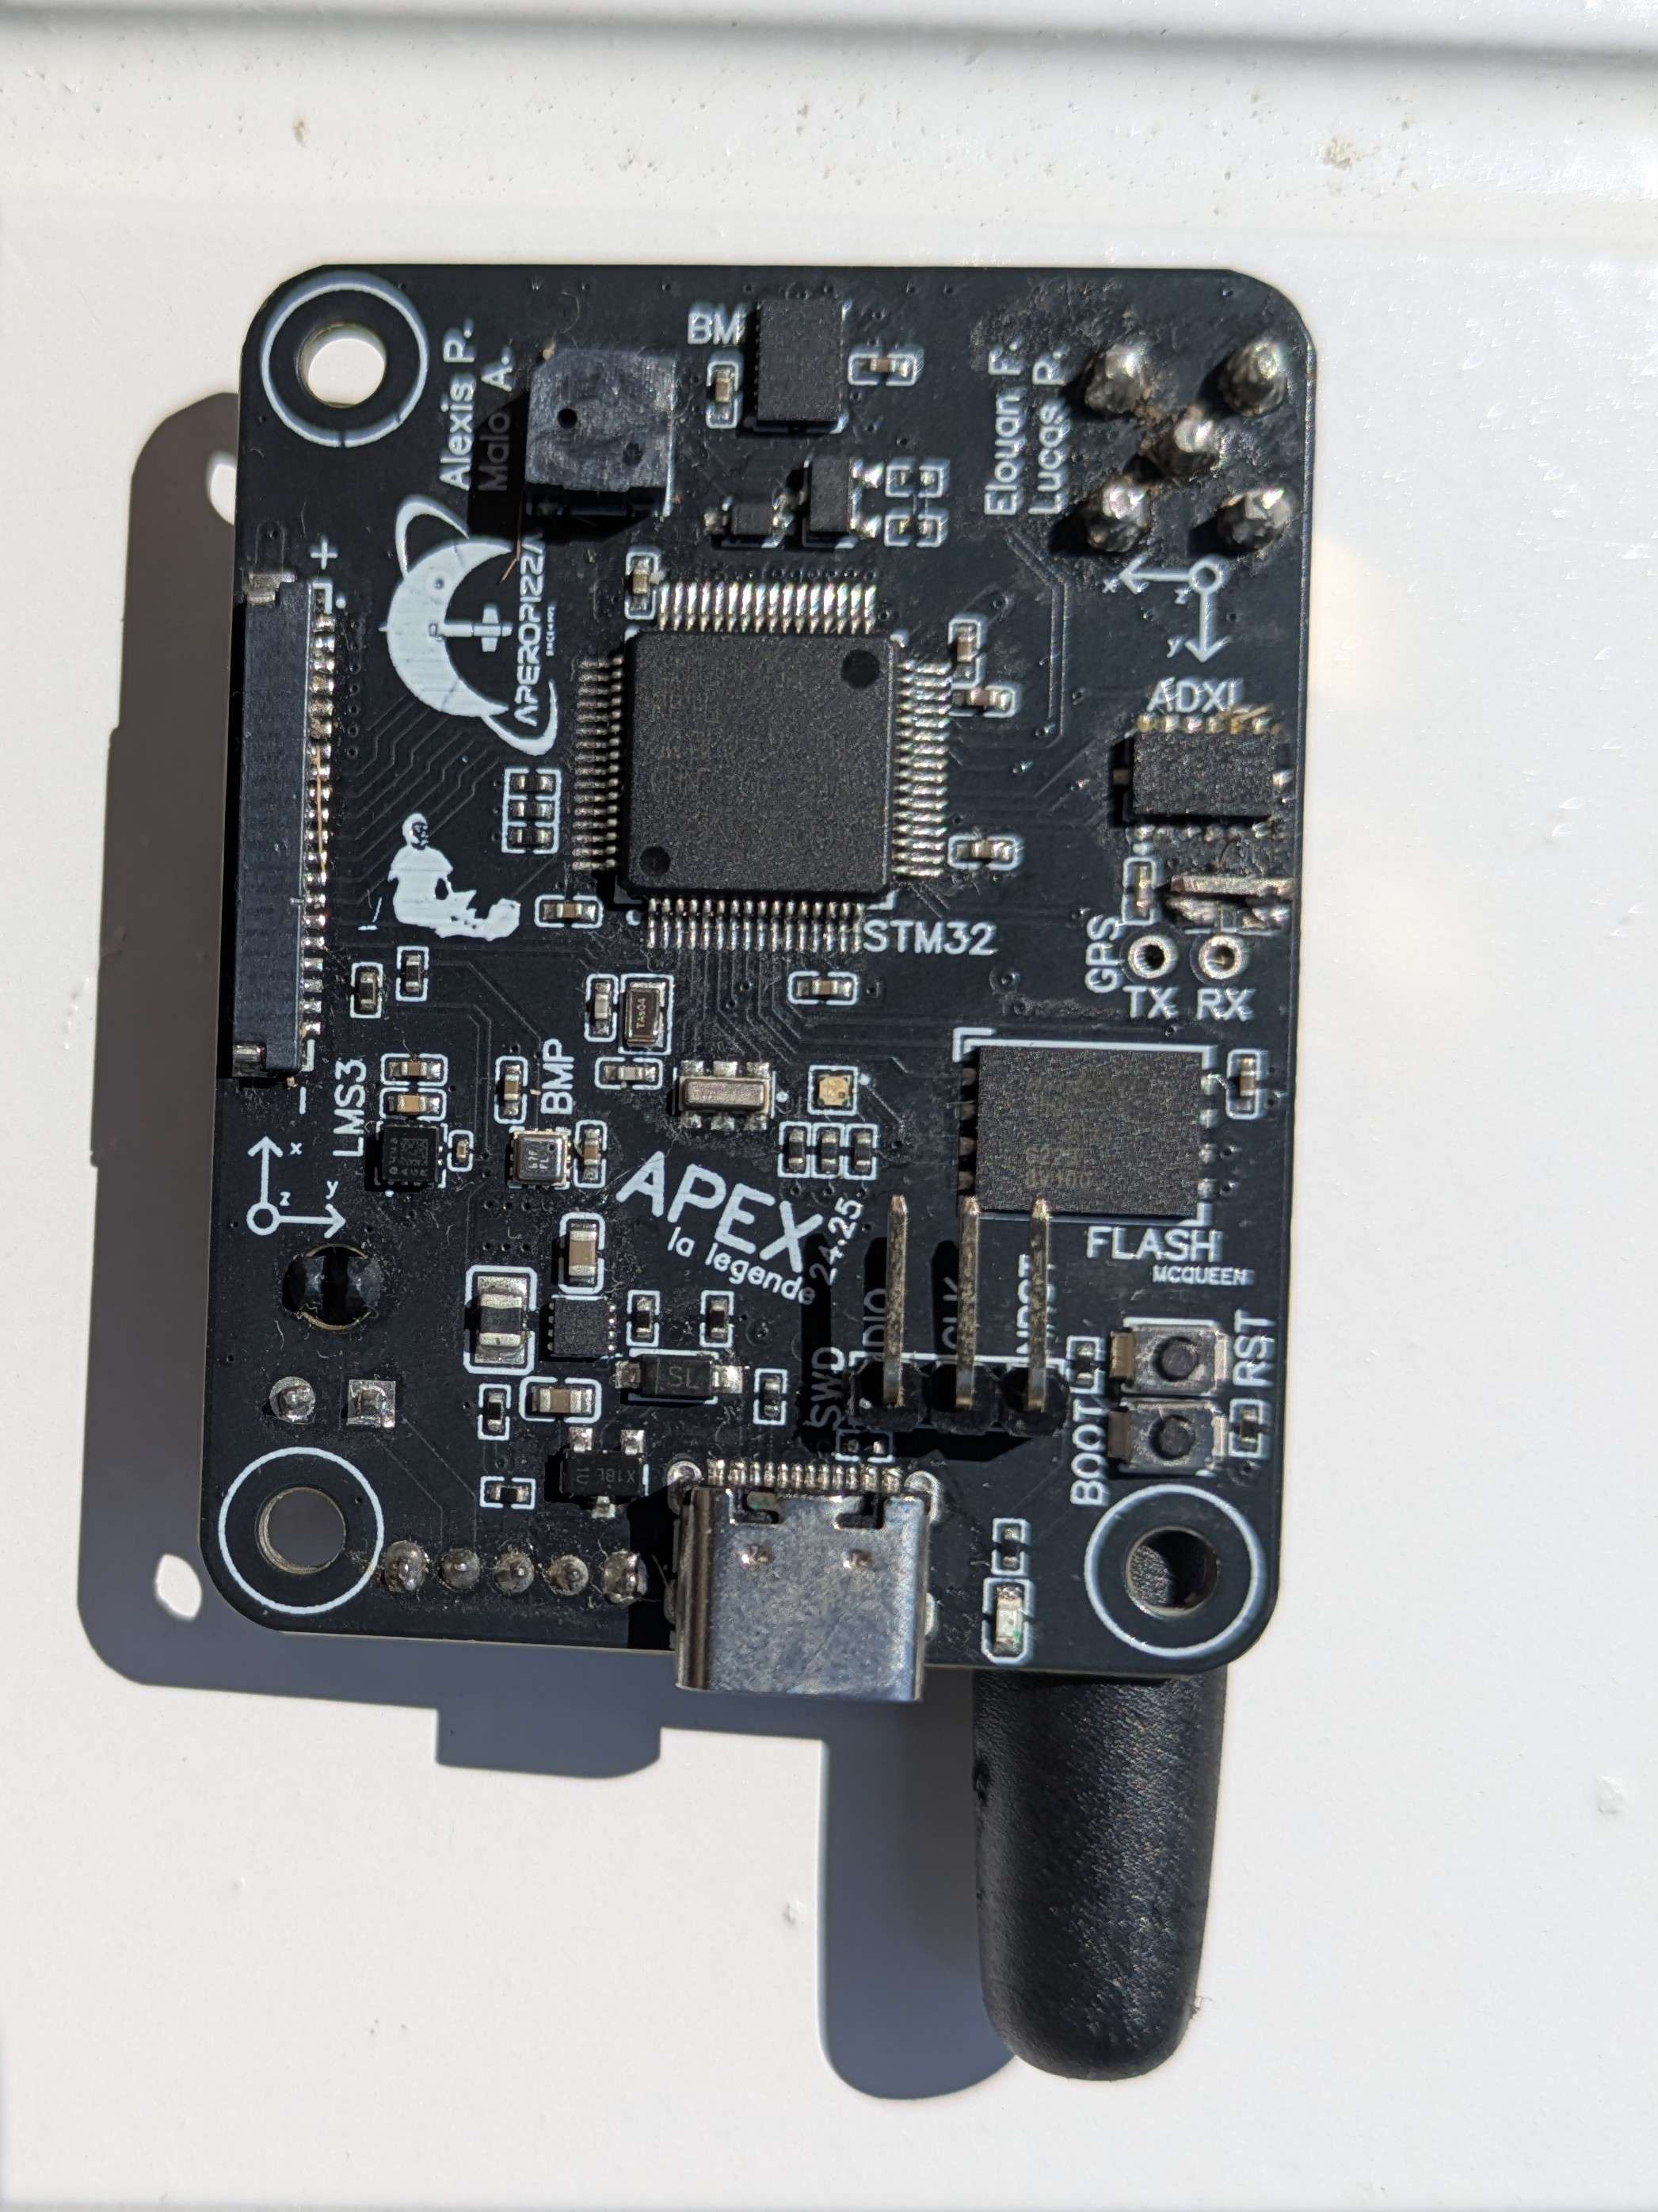
\includegraphics[width=0.70\textwidth]{image/APEX_FRONT.jpg}};

    \node (BMI_lbl) at (-4.00, +3.5) {BMI088};
    \node (Buz_lbl) at (-3.90, +3.0) {Buzzer};
    \node (ADX_lbl) at (-4.10, +2.5) {ADXL370};
    \node (STM_lbl) at (-3.90, +2.0) {STM32};
    \node (Con_lbl) at (-4.25, +1.5) {Connecteur};
    \node (W25_lbl) at (-4.30, +1.0) {W25Q512JV};
    \node (RGB_lbl) at (-4.30, +0.5) {LED RGB 0};
    \node (LSM_lbl) at (-4.35,  0.0) {LSM303AGR};
    \node (BMP_lbl) at (-4.00, -0.5) {BMP380};
    \node (SWD_lbl) at (-4.05, -1.0) {Pin SWD};
    \node (PW0_lbl) at (-4.15, -1.6) {Régulateur};
    \node (PW1_lbl) at (-4.10, -1.9) {de tension};
    \node (USB_lbl) at (-3.85, -2.5) {USB C};
    \node (LED_lbl) at (-4.15, -3.0) {LED PWR};
    \node (ATN_lbl) at (-4.00, -3.5) {Antenne};

    \node (BMI_box) at (-0.10, +2.50) [minimum width=03mm, minimum height=05mm, rectangle, fill=red, fill opacity=0.2] {};
    \node (Buz_box) at (-0.75, +2.30) [minimum width=05mm, minimum height=05mm, rectangle, fill=red, fill opacity=0.2] {};
    \node (ADX_box) at (+1.20, +1.10) [minimum width=05mm, minimum height=04mm, rectangle, fill=red, fill opacity=0.2] {};
    \node (STM_box) at (-0.25, +1.15) [minimum width=10mm, minimum height=10mm, rectangle, fill=red, fill opacity=0.2] {};
    \node (Con_box) at (-1.80, +0.95) [minimum width=04mm, minimum height=18mm, rectangle, fill=red, fill opacity=0.2] {};
    \node (W25_box) at (+0.90, -0.10) [minimum width=09mm, minimum height=06mm, rectangle, fill=red, fill opacity=0.2] {};
    \node (RGB_box) at (+0.01, +0.05) [minimum width=01mm, minimum height=01mm, rectangle, fill=red, fill opacity=0.2] {};
    \node (LSM_box) at (-1.40, -0.15) [minimum width=01mm, minimum height=01mm, rectangle, fill=red, fill opacity=0.2] {};
    \node (BMP_box) at (-0.97, -0.18) [minimum width=01mm, minimum height=01mm, rectangle, fill=red, fill opacity=0.2] {};
    \node (SWD_box) at (+0.45, -0.70) [minimum width=08mm, minimum height=08mm, rectangle, fill=red, fill opacity=0.2] {};
    \node (PW0_box) at (-0.70, -0.88) [minimum width=12mm, minimum height=10mm, rectangle, fill=red, fill opacity=0.2] {};
    \node (USB_box) at (-0.08, -1.60) [minimum width=09mm, minimum height=08mm, rectangle, fill=red, fill opacity=0.2] {};
    \node (LED_box) at (+0.60, -1.62) [minimum width=01mm, minimum height=05mm, rectangle, fill=red, fill opacity=0.2] {};
    \node (ATN_box) at (+0.90, -2.60) [minimum width=08mm, minimum height=13mm, rectangle, fill=red, fill opacity=0.2] {};

    \draw[red, ->] (BMI_lbl.0) -- (BMI_box.center);
    \draw[red, ->] (Buz_lbl.0) -- (Buz_box.center);
    \draw[red, ->] (ADX_lbl.0) -- (ADX_box.center);
    \draw[red, ->] (STM_lbl.0) -- (STM_box.center);
    \draw[red, ->] (Con_lbl.0) -- (Con_box.center);
    \draw[red, ->] (W25_lbl.0) -- (W25_box.center);
    \draw[red, ->] (RGB_lbl.0) -- (RGB_box.center);
    \draw[red, ->] (LSM_lbl.0) -- (LSM_box.center);
    \draw[red, ->] (BMP_lbl.0) -- (BMP_box.center);
    \draw[red, ->] (SWD_lbl.0) -- (SWD_box.center);
    \draw[red, ->] (PW0_lbl.-10) -- (PW0_box.center);
    \draw[red, ->] (USB_lbl.0) -- (USB_box.center);
    \draw[red, ->] (LED_lbl.0) -- (LED_box.center);
    \draw[red, ->] (ATN_lbl.0) -- (ATN_box.center);

\end{tikzpicture}
        \caption{Face avant du module APEX}
        \label{fig:apex_front}
    \end{subfigure}
    \begin{subfigure}{0.48\textwidth}
        \centering
\begin{tikzpicture}
    \node at (0, 0) {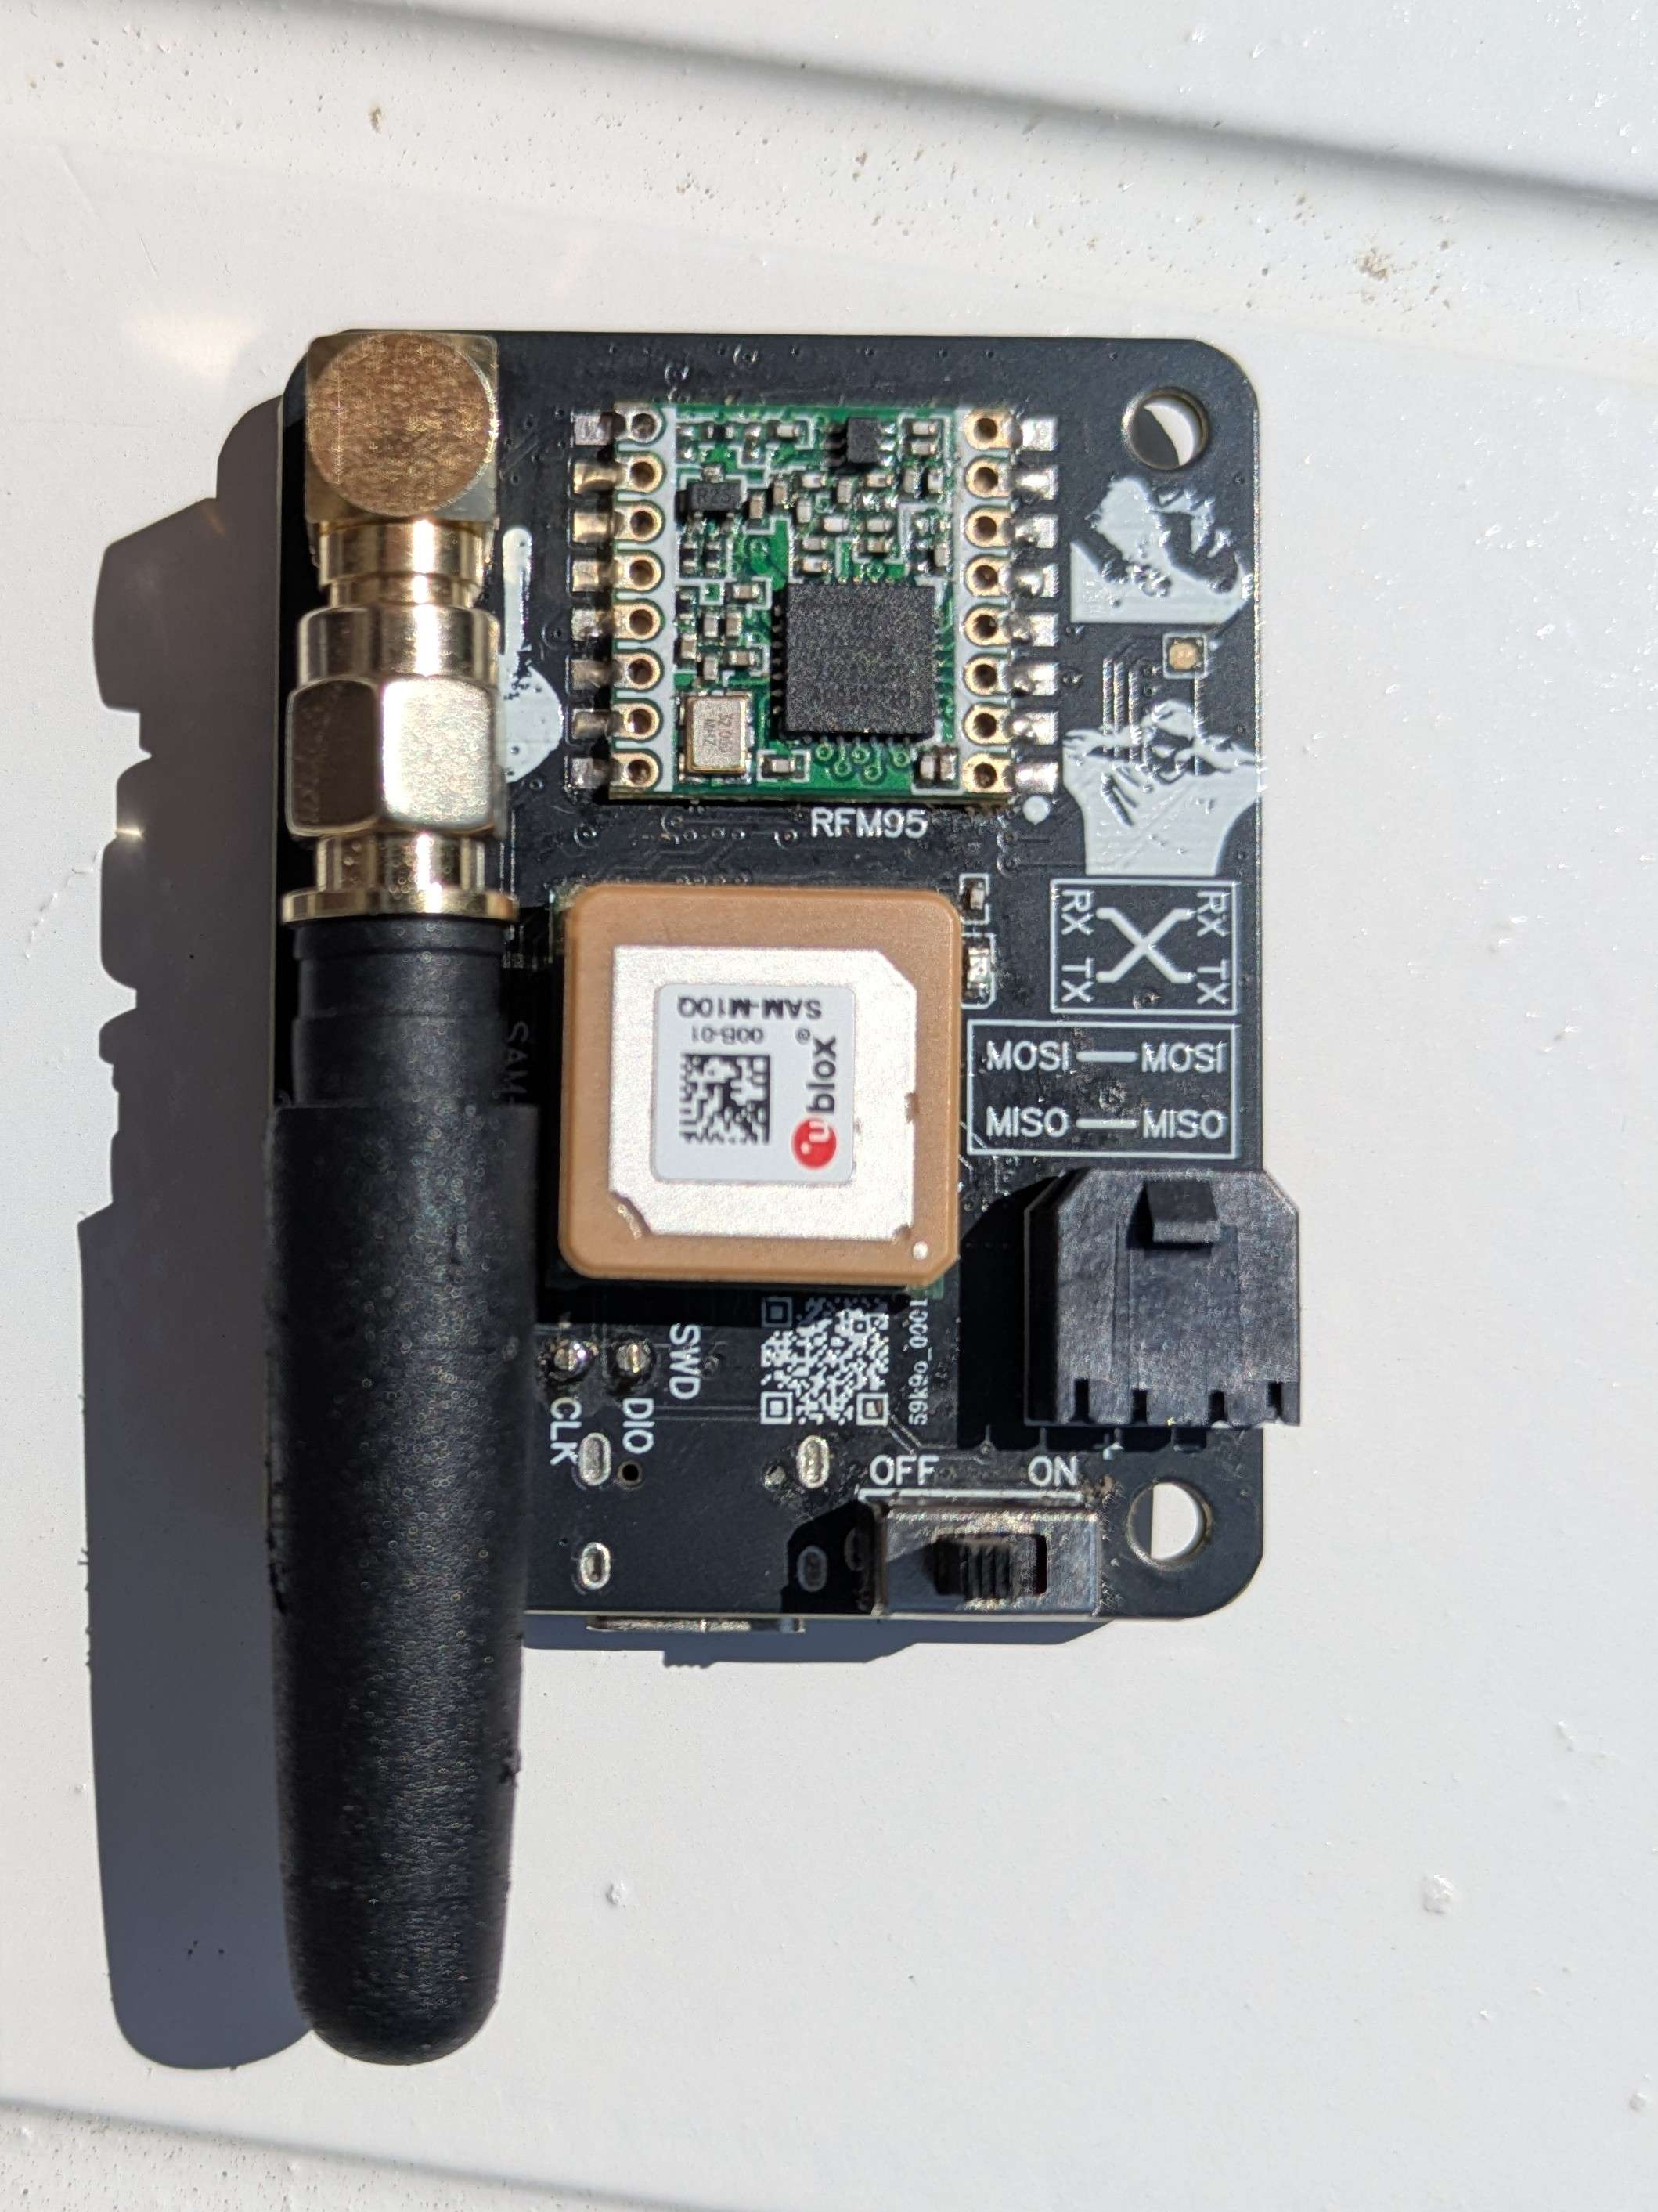
\includegraphics[width=0.70\textwidth]{image/APEX_BACK.jpg}};

    \node (RFM_lbl) at (3.80, +3.0) {RFM95W};
    \node (RBG_lbl) at (4.00, +2.0) {LED RGB 1};
    \node (GPS_lbl) at (3.95, +1.0) {SAM M10Q};
    \node (ANT_lbl) at (3.65,  0.0) {Antenne};
    \node (BT0_lbl) at (3.85, -0.8) {Connecteur};
    \node (BT1_lbl) at (3.60, -1.2) {batterie};
    \node (SW0_lbl) at (3.50, -2.0) {Switch};
    \node (SW1_lbl) at (4.10, -2.4) {d'alimentation};
    \node (SW2_lbl) at (3.60, -2.8) {batterie};

    \node (RFM_box) at (-0.05, +1.70) [minimum width=15mm, minimum height=15mm, rectangle, fill=red, fill opacity=0.2] {};
    \node (RBG_box) at (+1.19, +1.51) [minimum width=01mm, minimum height=01mm, rectangle, fill=red, fill opacity=0.2] {};
    \node (GPS_box) at (-0.23, +0.06) [minimum width=14mm, minimum height=14mm, rectangle, fill=red, fill opacity=0.2] {};
    \node (ANT_box) at (-1.40, -0.30) [minimum width=10mm, minimum height=60mm, rectangle, fill=red, fill opacity=0.2] {};
    \node (BT0_box) at (+1.16, -0.65) [minimum width=10mm, minimum height=10mm, rectangle, fill=red, fill opacity=0.2] {};
    \node (SW0_box) at (+0.55, -1.50) [minimum width=09mm, minimum height=05mm, rectangle, fill=red, fill opacity=0.2] {};

    \draw[red, ->] (RFM_lbl.180) -- (RFM_box.center);
    \draw[red, ->] (RBG_lbl.180) -- (RBG_box.center);
    \draw[red, ->] (GPS_lbl.180) -- (GPS_box.center);
    \draw[red, ->] (ANT_lbl.180) -- (ANT_box.center);
    \draw[red, ->] (BT0_lbl.-170) -- (BT0_box.center);
    \draw[red, ->] (SW1_lbl.180) -- (SW0_box.center);
\end{tikzpicture}
        \caption{Face arrière du module APEX}
        \label{fig:apex_back}
    \end{subfigure}
    \caption{Module APEX}
    \label{fig:apex}
\end{figure}

\subsection{Composants principaux}
\subsubsection{Microcontrôleur STM32F411RETx}
Le microcontrôleur STM32F411RETx est un microcontrôleur 32 bits de la famille STM32F4 de
STMicroelectronics. Il est basé sur un cœur ARM Cortex-M4 et dispose de 512 Ko de mémoire
flash, 128 Ko de SRAM et d'une fréquence d'horloge maximale de 100 MHz. Il est équipé de
multiples interfaces de communication, dont SPI, I2C, UART et USB, ainsi que de
multiples périphériques, tels que des convertisseurs analogique-numérique (ADC), des
convertisseurs numérique-analogique (DAC) et des timers. Le STM32F411RETx est
particulièrement adapté pour les applications embarquées nécessitant des performances
élevées et une faible consommation d'énergie. C'est le microcontrôleur STMicroelectronics
dont le compromis puissance / taille est le plus intéressant pour les applications
embarquées. Aussi, la documentation et les ressources disponibles pour ce
microcontrôleur ainsi qu'un environnement de développement complet et une communauté
active facilitent en font un choix intéressant pour les projets d'électronique
embarquée à l'association de l'AéroIPSA.\\

\subsubsection{Module de télémesure RFM95W}
Le module de télémesure RFM95W est un module de communication radio de la famille RMF9x
de HopeRF. Il permet une transmission de données sans fil de plusieurs modulations
différentes, dont le FSK, GFSK, MSK, GMSK, LoRa\texttrademark \ et OOK dans la bande de
fréquence 868/915 MHz\footnote{Il existe aussi les modules RFM96W et RFM98W qui
fonctionne avec les fréquences 169, 433 et 470 MHz.}. Ce module offre de nombreuse
fonctionnalitées et modes de fonctionnement. Cependant, pour ce projet, seuls les modes de
transmission et réception simples ont été utilisés.

\subsubsection{BMI088}

Le BMI088 est une central de mesure inertiel (IMU\footnote{\textit{Inertial Mesurment
 Unit} en anglais}) 6 DOF\footnote{\textit{Degree Of Freedom} en anglais} de Bosch
Sensortec (3 axes d'accélération et 3 axes de gyroscope). Il est conçu pour les
applications de haute performance et de faible consommation d'énergie. L'accéléromètre
offre différentes plage de mesure allant de $\pm 3g$ à $\pm 24g$ et le gyroscope de $\pm
125\degres/s$ à $\pm 2000\degres/s$ avec 16 bits de résolution ce qui fait une sensibilité de
$7\times10^{-4} g/LSB$ à $9\times10^{-5} g/LSB$. La fréquence d'actualisation
est au maximum de 1600 Hz pour l'accéléromètre et de 2000 Hz pour le gyroscope.\\

Pour ce projet, le BMI088 est utilisé pour mesurer les accélérations linéaires hors de la phase
propulsive de la fusée mais surtout les vitesses angulaire perrmettant un suivi d'attitude.

\subsubsection{ADXL370}

L'ADXL370 est un accéléromètre 3 axes de la famille ADXL3xx de Analog Devices. Il est
conçu pour les applications nécessitant une mesure de fortes accélérations à haute fréquence.
Il offre une plage de mesure fixe de $\pm 200g$ à une fréquence maximale de 3600 Hz et une
résolution de $16$ bits et donc une sensibilité de $6.1\times10^{-3} g/LSB$ ce qui est amplement
suffisant pour les applications de fusée amateur.

\subsubsection{LSM303AGR}

Le LSM303AGR est un capteur de mouvement 6 DOF de STMicroelectronics. Il combine un
accéléromètre 3 axes et un magnétomètre 3 axes dans un seul boîtier. L'accéléromètre
offre une plage de mesure de $\pm 2g$, $\pm 4g$, $\pm 8g$ ou $\pm 16g$ avec une résolution de 16
bits. Le magnétomètre quant à lui offre une plage de mesure de $\pm 50$ gauss avec la même
résolution de 16 bits. La fréquence d'actualisation maximale est de 100 Hz pour les deux
capteurs. Cette faible fréquence d'actualisation rend le LSM303AGR peu adapté pour mesurer les
accélérations durant la phase propulsive de la fusée. Cependant, c'est la mesure du champ
magnétique qui est intéressante dans le cadre de ce projet. En effet, le LSM303AGR permet
de mesurer le champ magnétique terrestre et donc, permet de réduire le phénomène de
dérive de l'attitude de la fusée durant le vol en corrigeant les mesures du BMI088.\\

\subsubsection{BMP380}

Le BMP380 est un capteur de pression barométrique de Bosch Sensortec. Il est conçu pour
les applications de mesure de pression atmosphérique et d'altitude. Il offre une plage de
mesure de pression de 900 hPa à 1100 hPa avec une résolution de 24 bits et une précision de
$\pm 8$ Pa soit $\pm 66$ cm. La fréquence d'actualisation maximale est de 200 Hz. Il est
également capable de mesurer la température avec une précision de $\pm 0.3$ °C.\\

Le BMP380 est utilisé pour mesurer la pression atmosphérique durant le vol de la fusée afin de
calculer l'altitude de la fusée. Il est également utilisé pour mesurer la température durant le
vol, pouvant être utile pour corriger les mesures de certains capteurs.

\subsubsection{W25Q512JV}

Le W25Q512JV est une mémoire flash NOR de Winbond. Il offre une capacité de 512 Mbits (64 Mo)
et est conçu pour les applications nécessitant un stockage de données non volatile. Il
dispose d'une interface SPI et permet des vitesses de lecture allant jusqu'à 104 MHz.\\

Le W25Q512JV est utilisé pour stocker les données collectées, calculées et reçues durant le vol
de la fusée.

\subsubsection{SAM M10Q}

Le SAM M10Q est un module GPS de u-blox. Il est composé d'une puce GPS M10 et d'une antenne
céramique. Il est conçu pour les applications nécessitant une localisation précise et
rapide. Il offre une précision de positionnement de l'ordre du mètre en conditions idéales et
une fréquence d'actualisation de 10 Hz. Il est également capable de recevoir des signaux
de nombreux systèmes de navigation par satellite, dont GPS, GLONASS, Galileo et BeiDou.\\

Le SAM M10Q est utilisé pour localiser la fusée durant son vol et ainsi permettre sa
relocalisation après son atterrissage. Il est également utilisé pour améliorer la précision
des mesures de positionnement et de vitesse en combinant les données du GPS avec celles
des autres IMU.

\newpage

\subsubsection{Connectivités}

Le module APEX dispose de plusieurs connectivités pour communiquer avec d'autres modules ou
organes de la fusée. Il dispose d'un connecteur USB-C pour la programmation et la
communication avec un ordinateur, d'un connecteur de débug SWD pour la programmation et le
débugage du microcontrôleur ainsi que d'un connecteur 20 pins pour connecter d'autres
modules ou capteurs.

\subsubsection{Alimentation}

Le module APEX est alimenté par une batterie LiPo 3.7V de 1000 mAh avec BMS\footnote{
\textit{Battery Management System} en anglais, permet de protéger la batterie contre les
surcharges, les décharges profondes et les courts-circuits} intégrée. APEX dispose d'un
régulateur de tension pour fournir une tension stable de 3.3V au microcontrôleur et aux
autres composants. Après expériences, la batterie de 1000 mAh permet de tenir au moins 7 heures,
sans connaitre la durée maximale. Le module peut également être alimenté par USB-C.

\subsubsection{Témoin utilisateur}

Le module APEX dispose de 5 témoins dont 3 programmable, une LED GPS et un témoin lumineux
d'alimentation. Le témoin d'alimentation est une LED rouge qui s'allume lorsque le module est
alimenté quelle que soit la source d'alimentation. La LED GPS est une LED rouge qui clignote
lorsque le module GPS a déterminé une position valide. Les 3 autres témoins programmables sont
deux LED RGB et un buzzer. Ils sont utilisés pour indiquer l'état du module, les erreurs ou les
événements importants durant le vol. Ils sont contrôlés par le microcontrôleur via une interface
\textit{PWM}\footnote{\textit{Pulse Width Modulation} en anglais, permet de générer un signal
numérique modulé en largeur d'impulsion} permettant la variation de l'intensité lumineuse des LED
et la fréquence du buzzer.\\

\newpage
\subsection{Conception du module}

\subsubsection{CAO - Conception Assistée par Ordinateur}

La conception du module APEX a été réalisée à l'aide du logiciel de CAO EasyEDA. Ce logiciel
permet de concevoir des schémas électroniques et de réaliser des routages de cartes
électroniques. Il dispose d'une bibliothèque de composants électroniques varié et est directement
intégré au service de fabrication de cartes électroniques JLCPCB. Il permet ainsi de concevoir
des cartes électroniques rapidement et de les faire fabriquer en ligne en ayant une vision
sur le catalogue de composants disponibles par JLCPCB.

\begin{figure}[h]
    \centering

    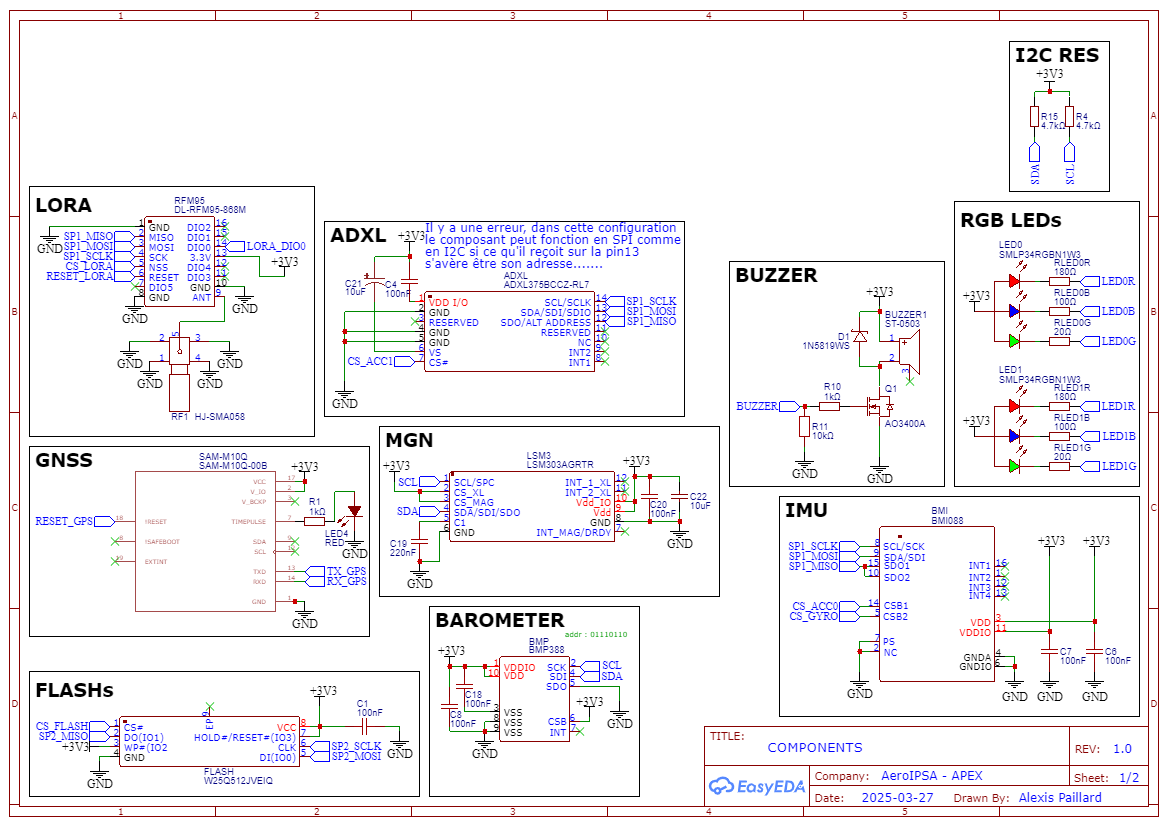
\includegraphics[width=0.75\textwidth]{image/Sheet_1.png}
    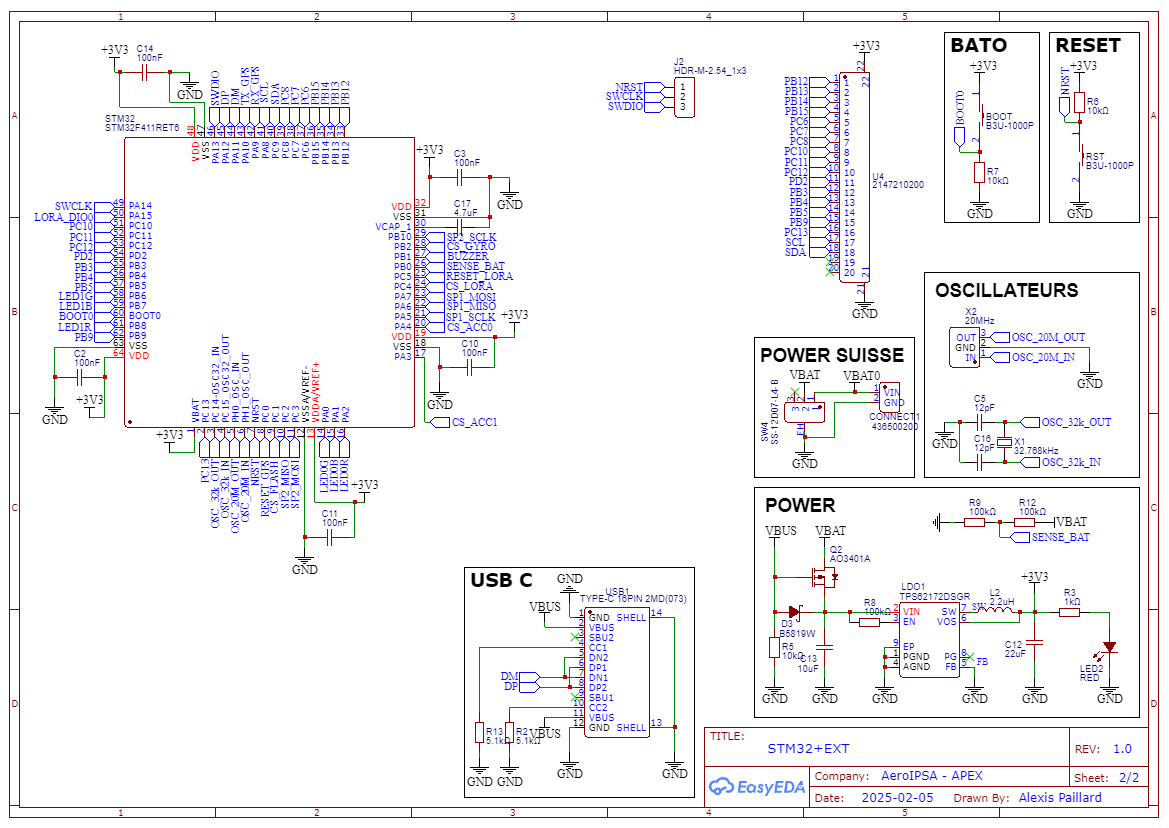
\includegraphics[width=0.75\textwidth]{image/Sheet_2.png}

    \caption{Schéma du module APEX}
    \label{fig:apex_schematic}
\end{figure}

Le schéma du module APEX est présenté dans la figure \ref{fig:apex_schematic}. Il est composé de
deux feuilles de schéma. La première feuille contient les principaux capteurs alors que la seconde
est dédiée au microcontrôleur, aux connectivités et à l'alimentation.

\newpage

Le routage du module APEX est présenté dans la figure \ref{fig:apex_routing}. Le module est
composé de 4 couches : une couche supérieure, une couche inférieure et deux couches
internes. La couche supérieure contient la majorité des composants soudés par l'entreprise
JLCPCB lors de la fabrication du PCB. La couche inférieure contient le module GPS, le module
de télémesure, l'antenne ainsi que d'autre composants mineurs. Ces composants sont soudés
manuellement après la réception du PCB. La couche interne 1 est dédiée aux pistes de
signaux et la couche interne 2 est dédiée à l'alimentation et à la moitié des signaux du
connecteur 20 pins. La masse est répartie sur toutes les couches zone de cuivre afin de
réduire les interférences électromagnétiques, d'améliorer la dissipation thermique et la
stabilité du signal.

\begin{figure}[h!]
    \centering
    \begin{subfigure}{0.40\textwidth}
        \centering
        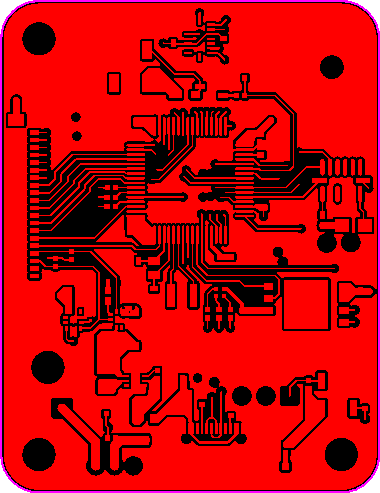
\includegraphics[width=\textwidth]{image/TopLayer.png}
        \caption{Couche supérieure}
        \label{fig:apex_top_layer}
    \end{subfigure}
    \begin{subfigure}{0.40\textwidth}
        \centering
        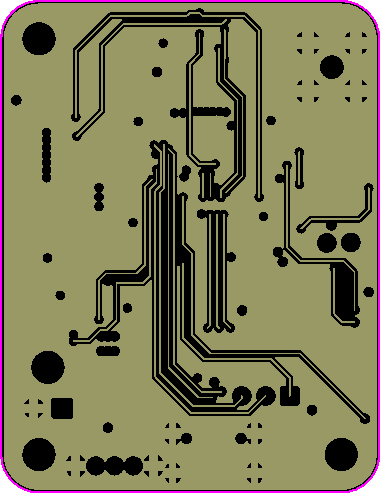
\includegraphics[width=\textwidth]{image/Inner1.png}
        \caption{Couche interne 1}
        \label{fig:apex_inner1}
    \end{subfigure}
    \begin{subfigure}{0.40\textwidth}
        \centering
        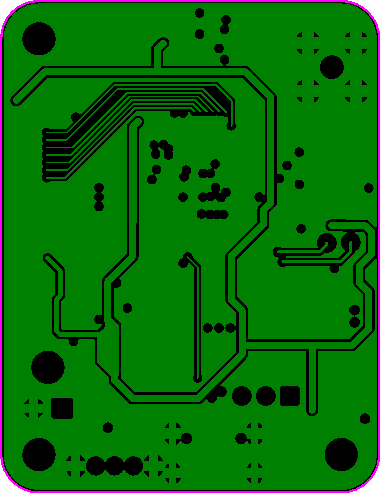
\includegraphics[width=\textwidth]{image/Inner2.png}
        \caption{Couche interne 2}
        \label{fig:apex_inner2}
    \end{subfigure}
    \begin{subfigure}{0.40\textwidth}
        \centering
        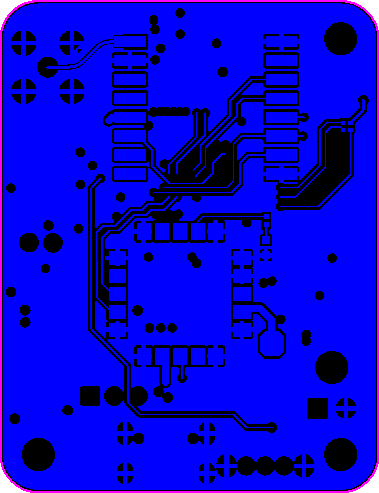
\includegraphics[width=\textwidth]{image/BottomLayer.png}
        \caption{Couche inférieure}
        \label{fig:apex_bottom_layer}
    \end{subfigure}
    \caption{Routage du module APEX}
    \label{fig:apex_routing}
\end{figure}

\newpage

\newpage

\subsection{Soudure des composants}

Comme dit précédemment, le module APEX a été fabriqué par l'entreprise JLCPCB avec la
majorité des composants de la couche supérieure soudés (hormis le buzzer et le connecteur
20 pins faute de disponiblité chez JLCPCB). Tous les autres composants se trouvant sur la
couche inférieure ainsi que le buzzer et le connecteur 20 pins ont été soudés manuellement
par les membres du projet. L'association de l'AéroIPSA dispose d'une plaque chauffante
permettant de souder les composants SMD\footnote{\textit{Surface-Mount Device} en anglais,
composants montés en surface} rapidement et efficacement. Elle a pu être utilisé pour
souder les composants de la couche supérieure. Cependant, la plaque chauffante ne
permet pas de souder les composants de la couche inférieure. En effet, la plaque
chauffante chauffe toute la carte électronique et cette dernière doit présenter une
surface plane pour être en contact avec la plaque chauffante. Il est donc impossible
d'effectuer une soudure une face par plaque chauffante lorsque des composants sont déjà
soudés sur l'autre face. Ainsi, les composants de la couche inférieure ont été soudés
manuellement à l'aide d'une station de soudure à air chaud.\\

La plus grande difficulté lors de la soudure des composants a été la soudure du module GPS
SAM M10Q. En effet, les pattes de ce module ne sont pas visible lorsque le module est
posé sur la carte électronique. Une erreur de positionnement du module de seulement
quelques millimètres ou la formation d'un pont de soudure entre deux pattes peut rendre le
module, et le plus souvent la carte électronique, inutilisable. De plus, des composants
interne du module GPS sont visible et à l'air libre sur la face inférieure du module. Il
est donc possible en appliquant trop de pâte à braser de faire un court-circuit entre ces
composants internes.\\

Sur les 4 modules APEX fabriqués, seule 2 cartes électroniques sont pleinement équipées
d'un module GPS fonctionnel:\\
\begin{itemize}
\item Une carte a été endommagée lors de l'alumage de la carte
électronique après soudure du module GPS, un court-circuit s'étant formé entre deux
pattes du module GPS et a surement endommagée l'un des cristals oscilateurs du module
ou le microcontrôleur interne. La carte APEX répondait toujours mais se mettait
immédiatement en défaut lors de son démarrage.\\
\item Sur une autre carte, le module GPS n'a jamais fonctionné. A chaque tentative
de soudure du module GPS, un court-circuit se formait entre deux pattes du module.
Expérience faite avec la précédente carte, et après plusieurs tentatives, de soudure /
déssoudure du module GPS, il a été décidé de laisser cette carte sans module GPS.
favorisant ainsi le bon fonctionnement des autres composants.\\
\end{itemize}

Ces problèmes de soudure du module GPS auraient pu être évités en mettant le GPS sur la
face supérieure de la carte électronique, la soudure à la plaque chauffante étant plus
facile. Cela aurait cependant impliqué de revoir le routage, la disposition et la taille
de la carte électronique ce qui n'était pas envisageable dans le cadre de ce projet.
Il aurait été également possible de demander à JLCPCB de souder l'intégralité des
composants, y compris ceux de la couche inférieure. Cependant, le coût de fabrication
de la carte électronique aurait été trop important, le budget d'une carte APEX étant
déjà conséquent.

\newpage

\subsection{Programmation du module APEX}

Un des retours d'expérience du projet Unknown était les faibles performances du programme
écrit. En effet, il n'était pas possible d'atteindre une fréquence d'échantillonnage
élevé et surtout stable. Le programme du projet APEX a donc été écrit de manière à
maximiser la rapidité d'exécution tout en gardant une modularité du code. Pour cela, et
dans une démarche d'apprentissage et d'approfondissement des connaissances en
programmation embarquée, la volonter a été de créer un système de moniteur temps
réel (RTOS\footnote{\textit{Real-Time Operating System} en anglais}) simple et adapté
aux besoins du projet. Ce RTOS permet de gérer la création de tâches et leur ordonnancement
non préemptif voulant s'approcher d'une syntaxe proche des conceptes de la programmation
asnychrones comme nous ponvons l'entendre dans les langages modernes.\\

Bien que la programmation de ce RTOS ait débuté dès le début du projet, il n'a pas pu être
finalisé et fiabilisé à temps pour être utilisé durant les vols. En effet, même si le projet
était bien avancé avant la campagne, un problème de fiabilité du code a été découvert lors des
tests finaux avant la campagne de lancement. Ainsi, il a été décidé d'utiliser un code plus
simple et plus fiable, écrit en C standard, pour les vols. Le RTOS sera finalisé et
fiabilisé pour de futurs projets.\\

Le code utilisé durant les vols est écrit en C standard et a dû être développé en moins de 2
jours afin d'être prêt pour le premier vol de Prisma. Il est donc simple, peu optimisé et ne
répondant à seulement une partie des objectifs initiaux.

\newpage

\section{Station sol APEX}

\subsection{Objectif du projet}

La station sol APEX a été pensée comme une solution modulaire, portable et durable,
réutilisable sur plusieurs années. Elle permet de recevoir et d'afficher en temps réel
les données transmises en LoRa par le module embarqué APEX. Elle a également été conçue
pour être compatible avec de futurs projets, en assurant la réception de leur télémesure
sans dépendre exclusivement du module APEX.

\subsection{Composition principale}

\begin{itemize}
    \item Raspberry Pi 5 : exécute Raspbian et notre logiciel de récupération et
    d'affichage des données.
    \item Module TTGO : réception des communications LoRa 868 MHz.
    \item Batterie : alimentation autonome pour les campagnes de lancement.
    \item Écran et clavier : interaction et consultation directe des données.
\end{itemize}

\subsection{Fonctionnement}

Lors d'un lancement, le module embarqué APEX transmet ses données de télémesure via LoRa à
868 MHz. L'antenne de la station sol capte ces signaux et les transmet au module TTGO, qui
joue le rôle de récepteur LoRa. Les trames ainsi reçues sont envoyées à la Raspberry Pi 5,
où un logiciel dédié décode et organise les informations. Les données sont ensuite affichées
en temps réel sur l'écran de la station sol, permettant aux opérateurs de suivre l'évolution
du vol (position GPS, altitude, capteurs embarqués, etc.). Grâce à cette architecture, la
station est portable, autonome et peut être facilement réutilisée pour d'autres projets de
télémesure.

\begin{figure}[h!]

    \centering
    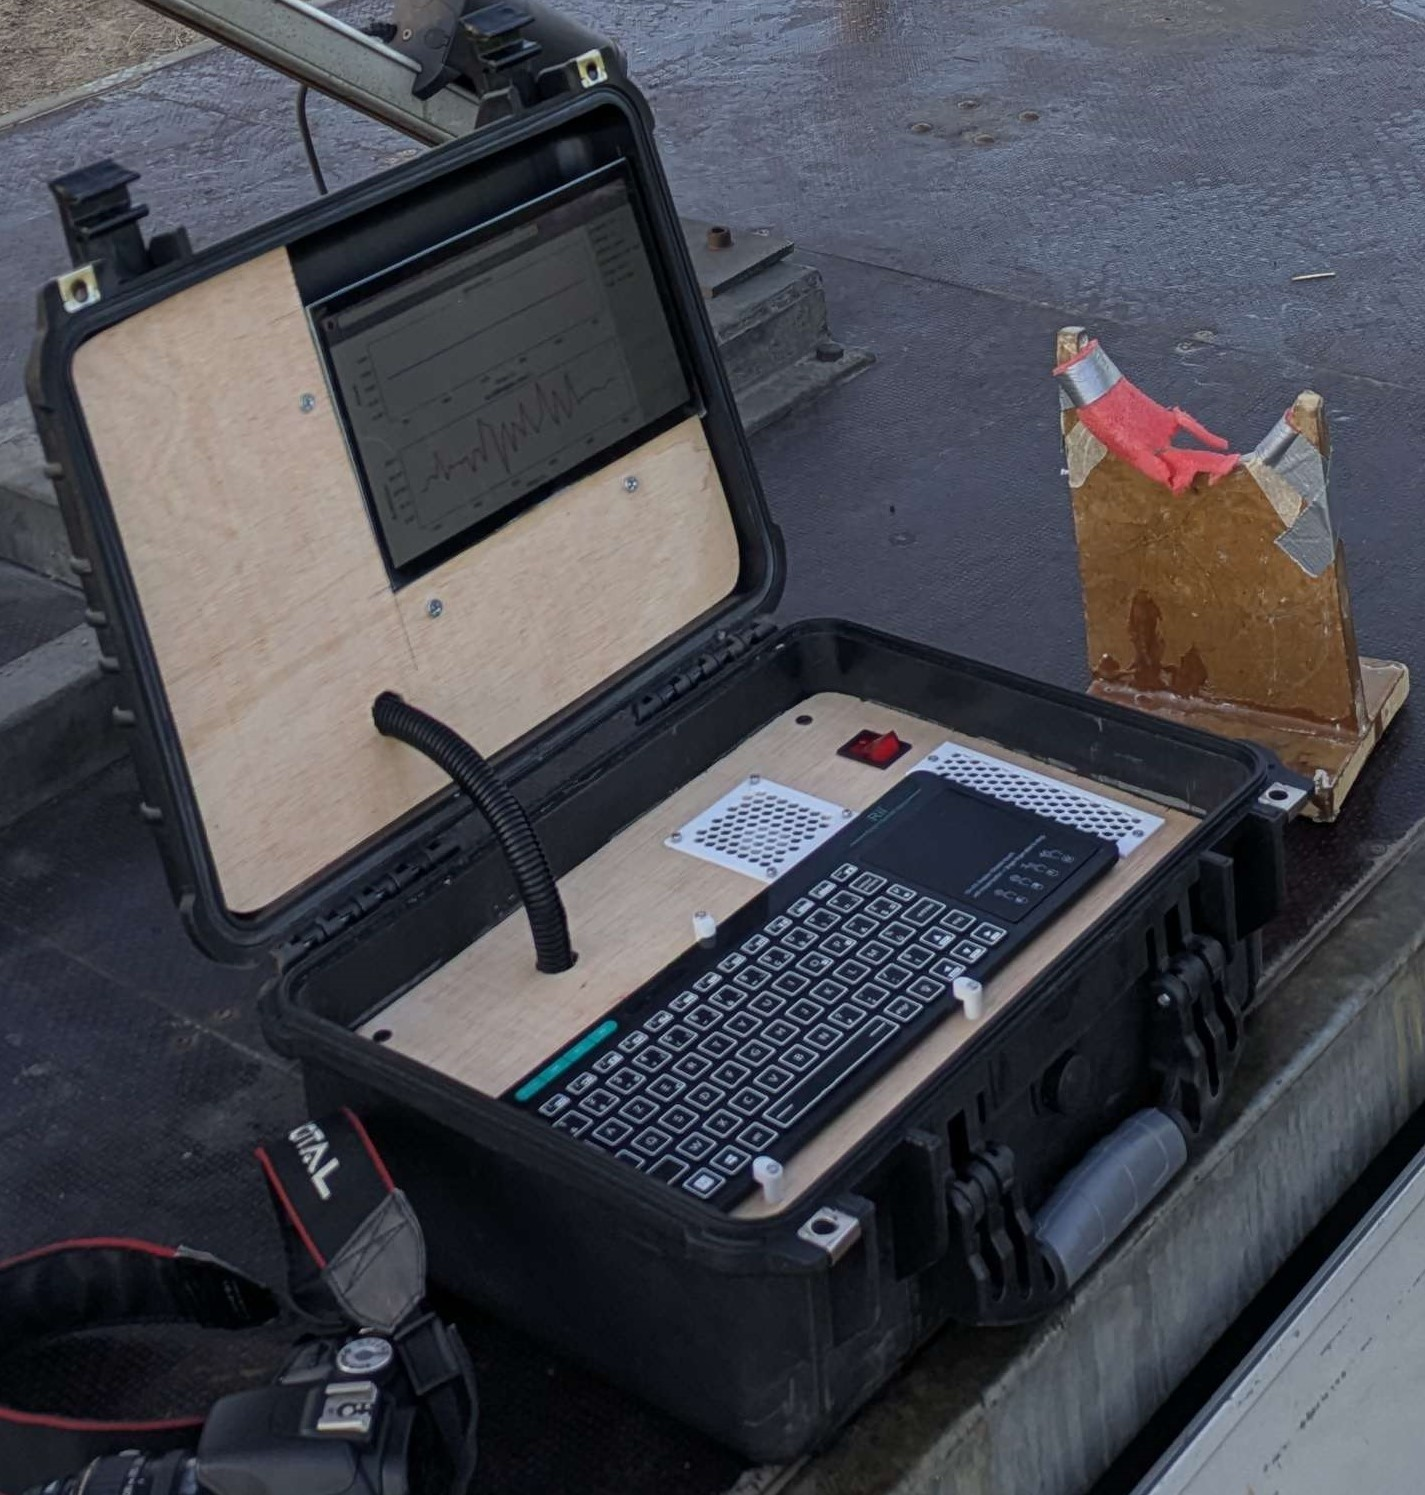
\includegraphics[width=0.75\textwidth]{image/station_sol_zoom.jpg}
    \caption{Station sol APEX}
    \label{fig:station_sol_apex}

\end{figure}

\newpage

\section{Expériences et résultats}

Le projet APEX s'est inscrit dans plusieurs projet de l'association de l'AéroIPSA de
l'année 2024-2025. Le module APEX a été embarqué sur une fusex\footnote{Fusée amateur
possédant un moteur de poussée équivalente ou supérieure à celui du moteur Pro54.} (MROM),
deux minif \footnote{Fusée amateur possédant le moteur Pro24 ou équivalent.} (Prisma et
Horizon) et un cansat\footnote{Micro-satellite atmosphérique le plus souvent largé par
une fusée dont le gabarit peut faire penser à une canette.} (Prisma). Cela explique le
nombre de 4 modules APEX commandés.\\

\subsection{Prisma}

Le premier vol du module APEX a eu lieu avec le projet Prisma. 2 modules APEX se trouvaient
à bord de Prisma, l'un dans la fusée et l'autre dans le cansat devant être largué par la
fusée à son apogée.\\

Le projet n'ayant pas inscrit la station sol APEX dans sa chronologie, la télémesure n'a pas
été utilisé durant le vol. Les données collectées par les modules APEX ont été stockées
et récupérées après le vol. Cependant, à cause d'une erreur de programmation, les données
ont été encryptées sur la mémoire flash des modules APEX d'une manière non prévue. Il n'a
donc pas été possible de récupérer les données collectées durant le vol.\\

Le vol de Prisma a tout de même permis de valider le bon fonctionnement du module APEX
dans un environnement de vol réel. Le module a parfaitement résisté aux vibrations et
accélérations subies durant le vol. Le module APEX a également parfaitement fonctionné
avant et après le vol, prouvant ainsi la robustesse du module et prouvant que la capacité
de la batterie est suffisante largement suffisante pour plusieurs heures de vol.

\subsection{Horizon}

Le projet Horizon a été le second projet de l'AéroIPSA à embarquer un module APEX. Le
module APEX embarqué dans la fusée Horizon n'était pas équipé d'un module GPS à cause
des problèmes de soudure évoqués précédemment et ne possédait pas non plus le même
type de connecteur batterie faute de disponibilité lors de la campagne de lancement.\\

Lors de l'allumage de la carte APEX, au moment de la chronologie de lancement, le module
ne s'est pas allumé correctement (pas de LED d'alimentation allumée et pas de témoin sonore).
Le lancement a quand même eu lieu puisque le projet APEX est indépendant du projet Horizon.\\

Après le vol, lorsque le module APEX a été récupéré, il a été constaté que le module s'était
allumé et que le placement des cables des caméras embarquées bloquaient la vue de la LED
d'alimentation. Cependant, aucune données n'a été collectée durant le vol. Nous pensons que
cela est du à un faux contact au niveau du connecteur de la batterie. Le module ne s'était
donc pas allumé comme dit précédemment et lors de l'atterrissage, le module s'est allumé et
n'a jamais réussi à collecter des données attendant le décollage de la fusée.\\

\subsection{MROM}

Le projet MROM a été le troisième projet de l'AéroIPSA à embarquer un module APEX. Le
module APEX embarqué dans la fusée MROM était pleinement fonctionnel et équipé d'un
module GPS. La station sol APEX a également été utilisée durant le vol de la fusée MROM.\\

Lors de l'allumage de la carte APEX, au moment de la chronologie de lancement, le module
s'est allumé correctement (LED d'alimentation allumée et témoin sonore). Au même moment,
la station sol APEX a également commencé à recevoir les données transmises par le module
validant ainsi le bon fonctionnement de la télémesure.\\

Lors du lancement de la fusée, la station sol APEX n'a pas afficher les données de
télémesure comme espéré. En effet, les accélération subies par la fusée durant la
phase propulsive n'ont pas été apperçu sur la station sol. Après analyse des données
collectées par le module APEX, il s'est avéré que le module a pourtant bien collecté
les données durant le vol. Un taux important de données enregistrées ont cependant été
corrompues et ce de manière fréquencé durant le vol. Nous pensons que cela est dû à une
mauvaise programmation du module. En ne prennant que les données valides il est possible
de retracer les accélérations et vitesses angulaires subies par la fusée durant le vol.\\

\newpage

Ci dessous se trouve un graphique présentant les accélérations transversales (X, Y, Z) ainsi
que les vitesses angulaires (X, Y, Z) mesurées par le module APEX durant le vol de la
fusée MROM. On peut bien distinguer la phase propulsive de la fusée durant laquelle les
accélérations et vitesses angulaires sont les plus importantes. On peut également distinguer
la phase de chute libre durant laquelle l'accélération longitudinale (Z) est minimale à la fin
de la phase propulsive (-2g) et remonte progressivement jusqu'à 0g. Durant cette phase de
chute libre, la vitesse angulaire longitudinale (Z) passe elle par un maximum et diminue
progressivement. Se suit après l'ouverture du parachute noté par une forte décélération, puis
une phase de descente sous parachute durant laquelle l'accélération longitudinale (Z) est
stable autour de -1g, et enfin l'atterrissage de la fusée noté par une forte accélération
suivie directement d'un plateau où toutes les valeurs n'ont plus aucune variation.

\begin{figure}[h!]
    \centering
    \begin{subfigure}{\textwidth}
        \centering
        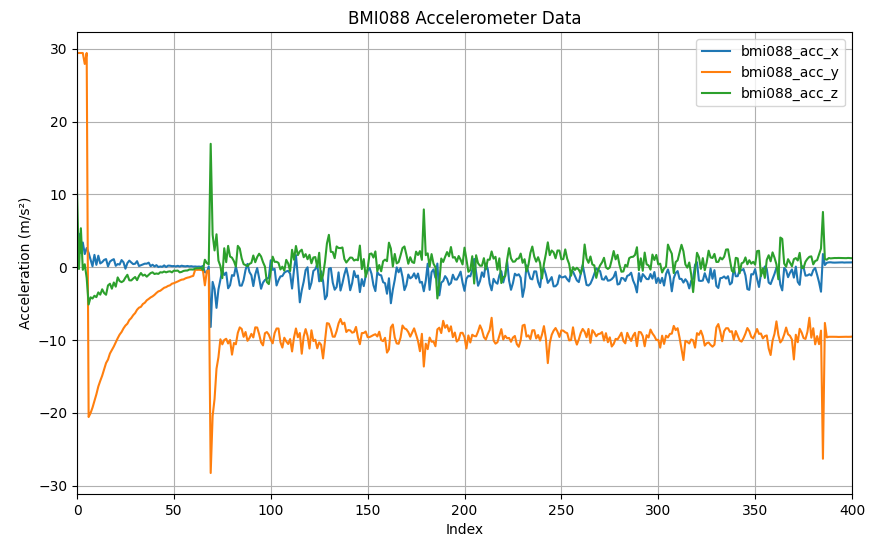
\includegraphics[width=0.8\textwidth]{image/MROM_acc.png}
        \caption{Accélérations de la fusée MROM}
        \label{fig:mrom_acc}
    \end{subfigure}
    \begin{subfigure}{\textwidth}
        \centering
        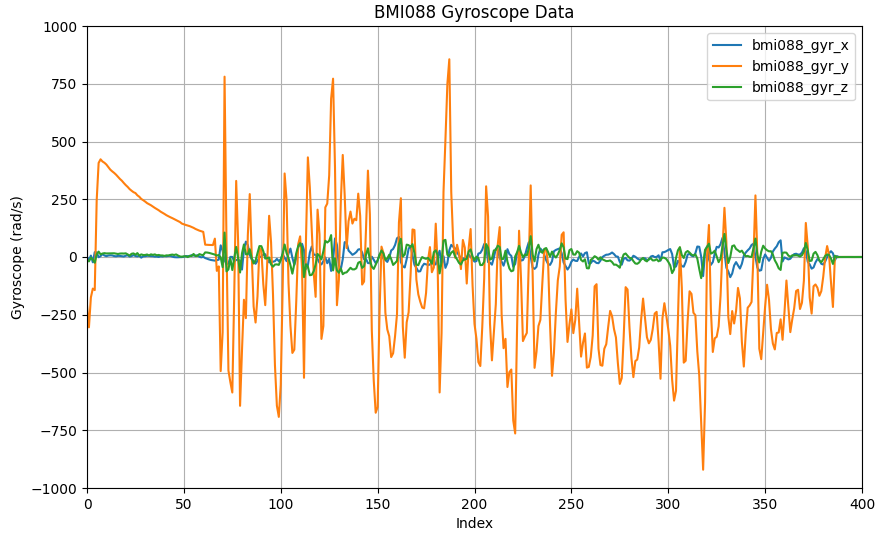
\includegraphics[width=0.8\textwidth]{image/MROM_gry.png}
        \caption{Vitesses angulaires de la fusée MROM}
        \label{fig:mrom_gyro}
    \end{subfigure}
    \caption{Données collectées par le module APEX durant le vol de la fusée MROM}
    \label{fig:mrom_data}
\end{figure}

Le maximum d'accélération longitudinale (Z) mesuré durant le vol est de 3g, ce qui est dû à une
erreur de programmation du module APEX. En effet, le module APEX a été programmé pour
mesurer des accélérations allant jusqu'à +-3g même si le BMI088 est capable de mesurer des
accélérations allant jusqu'à +-24g et que la fusée MROM est censée atteindre des
accélérations de l'ordre de 15g.

\newpage

\section*{Conclusion}

Le projet APEX a constitué une étape déterminante dans la continuité des travaux
réalisés au sein de l’AéroIPSA. Conçu comme une amélioration du module
\textit{Unknown}, il a permis d’apporter des solutions techniques plus abouties
et de relever de nouveaux défis dans le domaine de l’électronique embarquée
et des systèmes de télémesure. L’objectif principal était de développer un
module à la fois compact, performant et modulaire, capable de collecter un
ensemble élargi de données et de les transmettre efficacement à une station sol
réactualisée.\\

L’ensemble des travaux réalisés a permis de valider plusieurs points essentiels.
Sur le plan matériel, le développement d’une carte unique intégrant l’ensemble
des composants nécessaires au fonctionnement du module a représenté un véritable
progrès en termes d’intégration et de fiabilité. Sur le plan logiciel, une
attention particulière a été portée à l’optimisation du code et à la mise en
place de structures modulaires garantissant à la fois performance et évolutivité.
Enfin, la nouvelle station sol a marqué une avancée majeure en termes d’ergonomie
et de fonctionnalités, puisqu’elle est désormais capable de recevoir et
d’afficher les données de manière claire et réutilisable dans le cadre
d’autres projets de l’association.\\

Cependant, ce projet a également mis en lumière un certain nombre de limites et
d’axes d’amélioration. La complexité croissante des systèmes embarqués implique
des temps de développement plus longs et une phase de test particulièrement
exigeante. De plus, certaines fonctionnalités envisagées, comme l’optimisation
ultime de la fréquence d’échantillonnage ou l’intégration de nouveaux protocoles
de communication, n’ont pas encore atteint leur plein potentiel et devront être
poursuivies par les prochaines équipes.\\

Au-delà de ses résultats techniques, APEX illustre parfaitement l’importance de
l’apprentissage par projet. Chaque membre de l’équipe a pu approfondir ses
connaissances en électronique, en programmation embarquée, en communication
sans fil et en traitement de données, tout en développant des compétences
transversales essentielles telles que la gestion de projet, le travail
d’équipe et la résolution collective de problèmes complexes. L’expérience
humaine a ainsi été aussi riche que les progrès technologiques obtenus.\\

En définitive, APEX ne constitue pas un aboutissement, mais bien une étape dans
le processus d’amélioration continue des moyens techniques de l’AéroIPSA.
L’existence désormais d’un module fiable, modulable et réutilisable ouvre la
voie à de nouvelles expérimentations, qu’il s’agisse de l’ajout de capteurs
plus performants, de l’intégration de protocoles de communication innovants,
ou encore du développement d’outils logiciels permettant une exploitation
plus poussée des données recueillies. Le projet représente ainsi un socle
solide sur lequel les prochaines générations d’étudiants pourront s’appuyer
et constitue une contribution durable à l’évolution des projets de fusées
expérimentales menés au sein de l’association.

\end{document}
